\documentclass[10pt]{beamer}

\usetheme[progressbar=frametitle]{metropolis}

\usepackage[utf8]{inputenc}
\usepackage[export]{adjustbox}
\usepackage[french]{babel}
\usepackage[scale=2]{ccicons}
\usepackage{booktabs}
\usepackage{color, colortbl}
\usepackage{graphicx}
\usepackage{hyperref}
\usepackage{longtable}
\usepackage{multicol}
\usepackage{multirow}
\usepackage{pgfplots}
\usepackage{pifont}
\usepackage{smartdiagram}
\usepackage{subcaption}
%\usepackage{subfig}
\usepackage{tabularx}
\usepackage{tikz}
\usepackage{url}
\usepackage{wrapfig}
\usepackage{xcolor}
\usepgfplotslibrary{dateplot}
\usesmartdiagramlibrary{additions}
\usepackage{fancyqr}

\usepackage{xspace}
\newcommand{\themename}{\textbf{\textsc{metropolis}}\xspace}

\title{Do we need pre-processing in NLP ? } %\newline (au moins sur les données textuelles)}
\title{Pour en finir avec le pré-traitement des données textuelles ?}

%\subtitle{A modern beamer theme}
\date{January 21st 2026}
\author{Gaël Lejeune (\texttt{gael.lejeune@sorbonne-universite.fr})}
\institute{Sorbonne Université}
 \titlegraphic{
\hfill
\includegraphics[height=1.2cm]{images/STIH.png}
\hfill
\includegraphics[height=1cm]{./images/sorbonne.png}
\hfill
\includegraphics[height=1.2cm]{images/logo-dimeco.png}
\hfill
}
\usepackage{array}
\metroset{block=fill}

\begin{document}

\maketitle


%
\section{Les pré-traitements en TAL, what is it good for ?}

\begin{frame}{Le dogme}

\begin{figure}
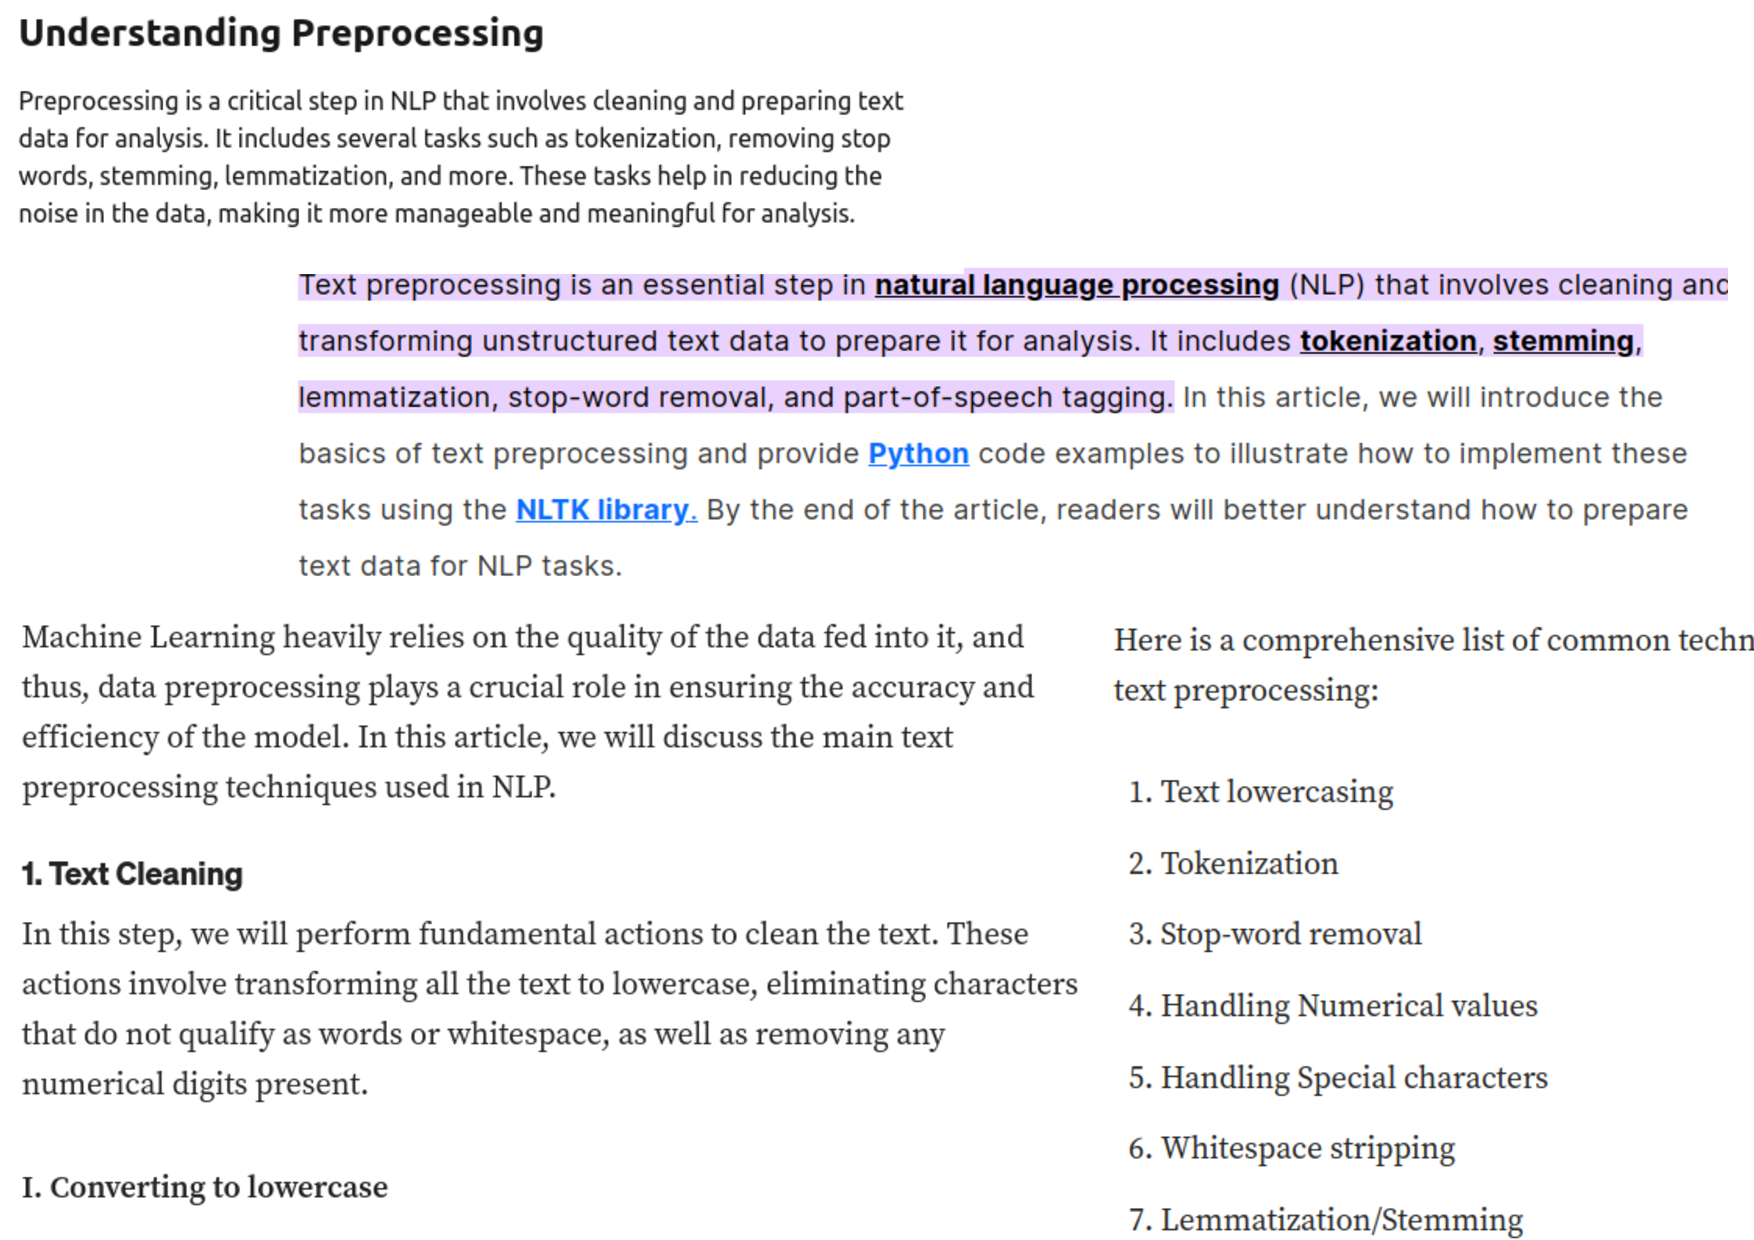
\includegraphics[width=1\textwidth]{./images/preprocess.pdf}
\end{figure}


\end{frame}

%%\begin{frame}{Plan}
%%\tableofcontents
%%\end{frame}

%%Les sections ça fait despetites transitions

\begin{frame}{Traitements ou pré-traitements}

\begin{block}{Quelle est la différence}
\begin{itemize}
\item Les pré-traitements sont anodins (mais obligatoires ?)
\item Les "traitements" sont plus nobles ?
\pause
\item Lesquels sont documentés et justifiés
\end{itemize}
\pause
Les pré-traitements sont en fait des traitements à part entière puisqu'ils ont un impact non nul sur les opérations subséquentes réalisées \cite{Millour-2020}

\pause
D'un point de vue de conception :
\begin{itemize}
  \item Ils prennent du temps
  \item Focalisent-il l'attention sur les bons problèmes ?
\pause
  \item Améliorent-ils les résultats ?
\end{itemize}
\pause
\end{block}

\end{frame}

\begin{frame}{De quels pré-traitements parle-t-on ?}

\textit{In the literature there is no convention adopted, and each work tests some preprocessing techniques rather than others.}%\footnote{}

\begin{itemize}
\item Lowercase letters.
\item Spelling Correction.
\pause
\item Removing HTML tags/ URLs.
\pause
\item Removing punctuation.
\item Removing stop words
\pause
\item Removing Emojies
\pause
\item Tokenization
\item Stemming 
\item Lemmatization
\end{itemize}
\pause
	\footnotesize{
How good is your tokenizer? on the monolingual performance of multilingual language models \cite{Rust-2020}

Stemming impact on arabic text categorization performance: A survey (Al Anzi 2015)

	\textbf{Is text preprocessing still worth the time? A comparative survey on the influence of popular preprocessing methods} \dots \cite{Siino-2024}
	}
%	\textbf{Is text preprocessing still worth the time? A comparative survey on the influence of popular preprocessing methods on Transformers and traditional classifiers} Siino et al. 2024
\end{frame}

\begin{frame}{Etat des lieux plus précis (Siino et al.)}
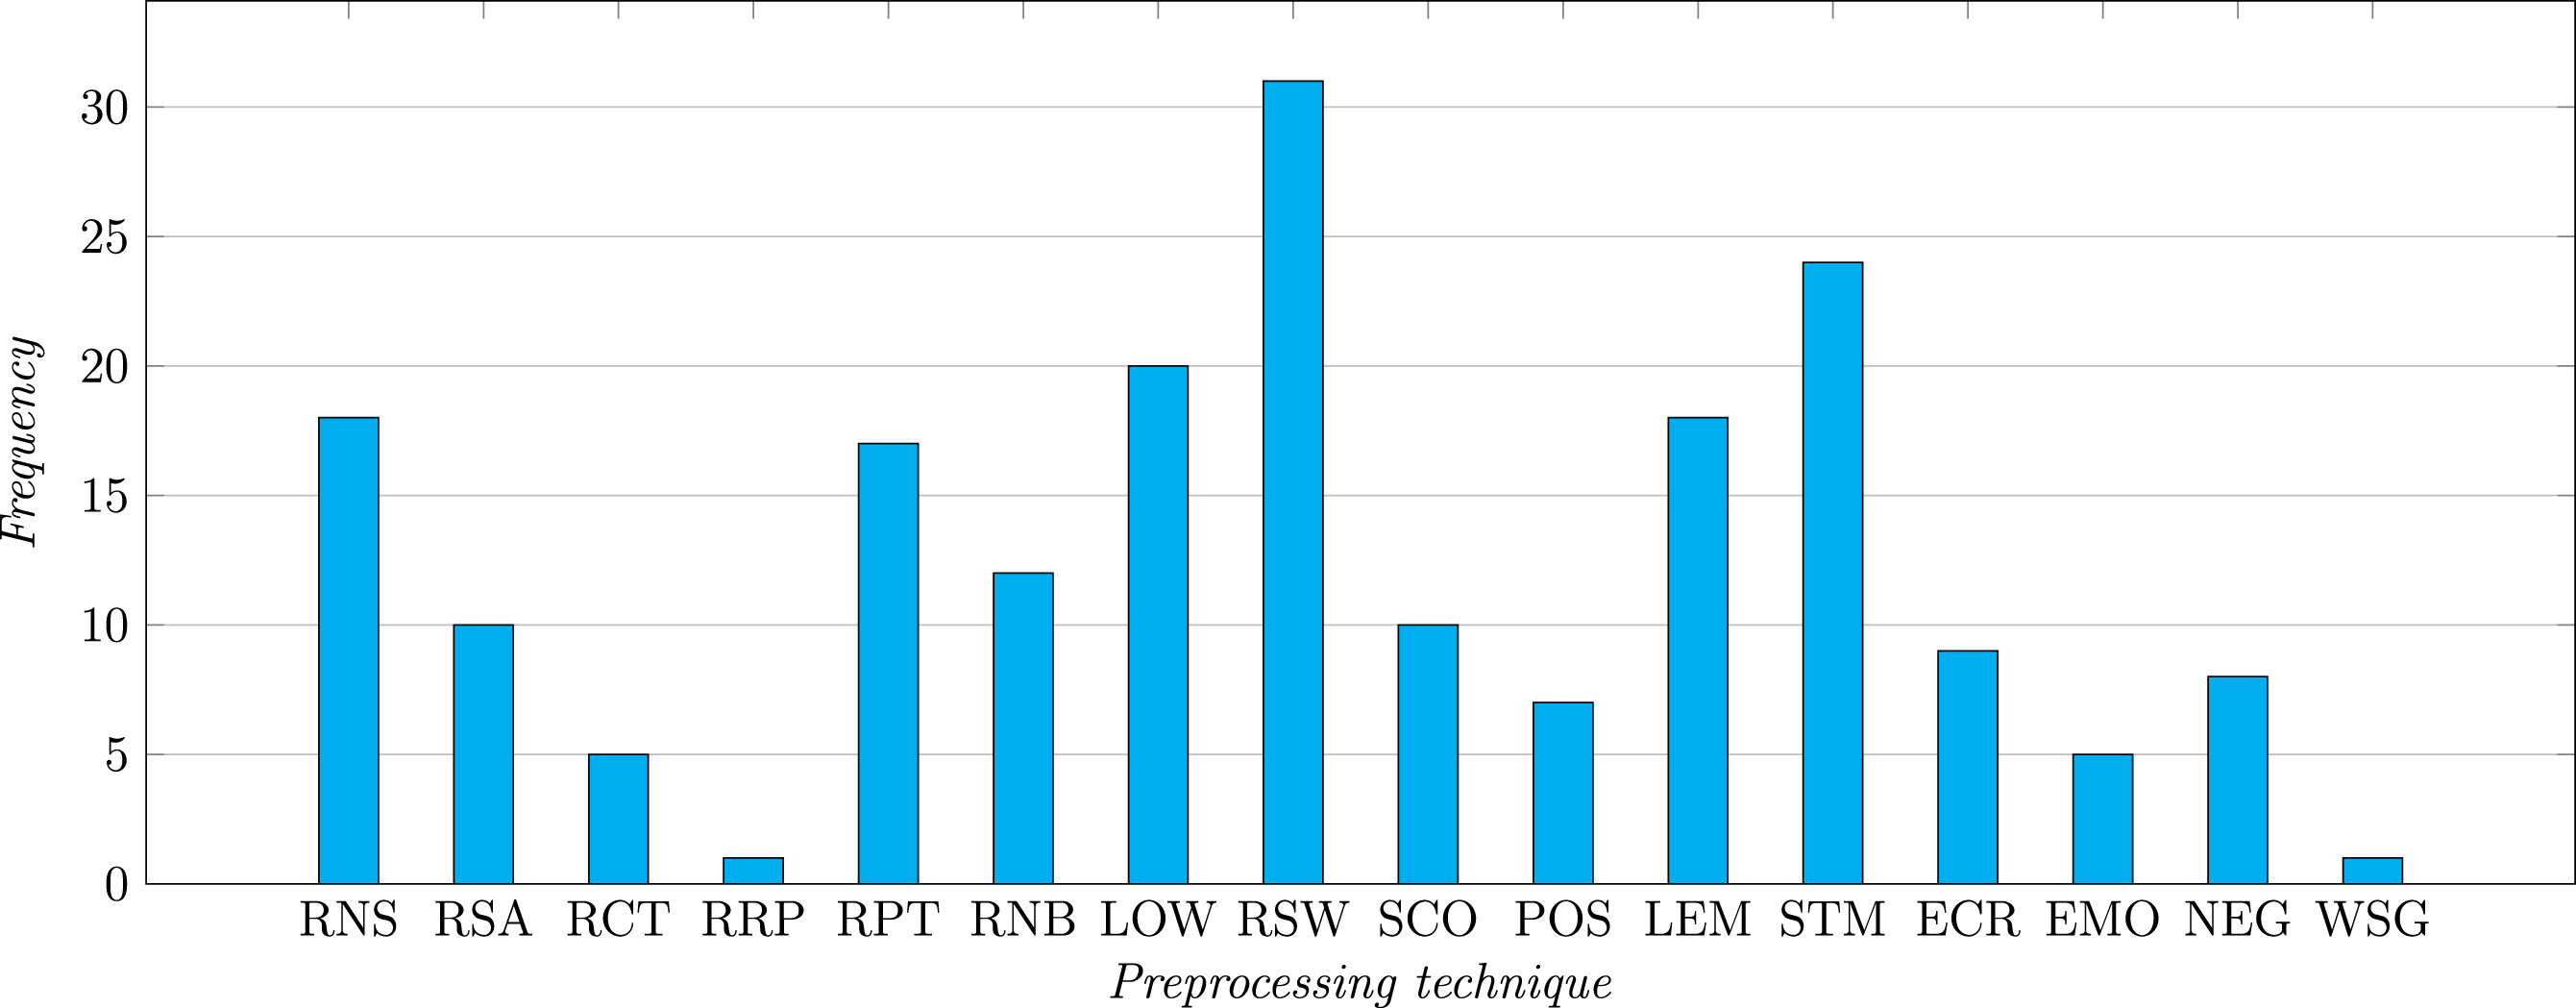
\includegraphics[width=.7\textwidth]{./images/preprocess_stats.png}
\begin{table}
\begin{tabular}{llll}
\textbf{ DON }&{ Do Nothing }&\textbf{  SCO }&{ Spelling Correction }\\
\textbf{ RNS }&{ Replace Noise }&\textbf{  POS }&{ Part-of-Speech Tagging }\\
\textbf{ RSA }&{ Replace Slang/Abbreviations }&\textbf{  LEM }&{ Lemmatization }\\
\textbf{ RCT }&{ Replace Contraction }&\textbf{  STM }&{ Stemming }\\
\textbf{ RRP }&{ Remove Repeated Punctuation }&\textbf{  ECR }&{ Remove Elongation }\\
\textbf{ RPT }&{ Removing Punctuation }&\textbf{  EMO }&{ Emoticon Handling }\\
\textbf{ RNB }&{ Remove Numbers }&\textbf{  NEG }&{ Negation Handling }\\
\textbf{ LOW }&{ Lowercasing }&\textbf{  WSG }&{ Word Segmentation  }\\
\textbf{ RSW }&{ Remove Stop Words }&\textbf{   }&{(sometrendingtopic)  }\\

\end{tabular}
\end{table}


\end{frame}

\begin{frame}{Polarité Critiques \texttt{en} (Siino et al.)}
\begin{figure}
\includegraphics[width=.6\textwidth]{./images/Res_siino.png}
\caption{Médiane de l'exactitude (\textit{accuracy}) sur 5 runs + diffmax. Pour chaque modèle le meilleur résultat est en gras, le pire en rouge}
\end{figure}
\end{frame}

\begin{frame}{Etat des lieux plus précis (\texttt{en}) (Siino et al.)}
IMDB: Polarité Critiques, PCL: Langage Condescendant Presse

FNS: AA Fake News, 20N: Catégorisation Forums
\includegraphics[width=.6\textwidth]{./images/Res_siino2.png}
\end{frame}

\begin{frame}{Langage Figuratif Tweets  \texttt{fr} \cite{Choi-2020}}
\begin{table}
\begin{scriptsize}
%\begin{tabular}{|l|p{.5cm}|p{.5cm}|l|l|l|l|l|l|l|l|}
\begin{tabular}{|l|p{.5cm}|p{.5cm}|p{.5cm}|p{.5cm}|p{.5cm}|p{.5cm}|p{.5cm}|p{.5cm}|p{.5cm}|p{.5cm}|}
\hline
 & \multicolumn{2}{l|}{\textbf{\begin{tabular}[c]{@{}l@{}}Logistic \\ Regression\end{tabular}}} & \multicolumn{2}{l|}{\textbf{Decision Tree}} & \multicolumn{2}{l|}{\textbf{MNB}} & \multicolumn{2}{l|}{\textbf{KNN}} & \multicolumn{2}{l|}{\textbf{Random Forest}} \\ \hline
 & \textbf{Count} & \textbf{Tfidf} & \textbf{Count} & \textbf{Tfidf} & \textbf{Count} & \textbf{Tfidf} & \textbf{Count} & \textbf{Tfidf} & \textbf{Count} & \textbf{Tfidf} \\ \hline
\textbf{DON} & \textbf{50.20\ } & \textbf{52.03 } & \textbf{50.41 } & \textbf{42.89 } & \textbf{51.42 } & \textbf{52.24 } & \textbf{38.82 } & \textbf{45.73 } & \textbf{53.25 } & \textbf{51.22 } \\ \hline
\textbf{RPT} & 50.41  & 52.64  & 48.37 & 44.72  & 50.81  & 51.63  & 38.21  & 45.53 & \textbf{\color{blue}53.05}  & \textbf{\color{blue}52.64}  \\ \hline
\textbf{RSW} & \textbf{\color{blue}52.24 } & 53.86  & 45.93  & 44.11  & 51.22  & 52.24  & 37.40  & 44.31  & 50.00  & 50.20  \\ \hline
\textbf{ACC} & 49.59  & 52.64  & 49.39  & 43.29 & 51.02  & 52.03  & 35.16  & 45.53  & 52.44  & 52.03  \\ \hline
\textbf{\color{red}\textbf{URL}} & \textbf{\color{red}47.56 } & \textbf{\color{red}47.36 } & \textbf{\color{red}39.43 } & \textbf{\color{red}39.43 } & \textbf{\color{red}50.20 } & \textbf{\color{red}50.61 } & \textbf{\color{red}34.35 } & \textbf{\color{red}41.46 } & \textbf{\color{red}45.53 } & \textbf{\color{red}44.51 } \\ \hline
\textbf{\color{blue}\textbf{LEM}} & 50.20  & \textbf{\color{blue}54.07 } & \textbf{\color{blue}49.19}  & 44.72 & \textbf{\color{blue}52.24 } & \textbf{\color{blue}53.25 } & \textbf{\color{blue}39.02 } & 45.53  & 50.41  & 51.63  \\ \hline
\textbf{STM} & 51.63  & 53.86  & 48.37 & \textbf{\color{blue}45.93}  & 52.03  & 52.44 & 38.41  & \textbf{\color{blue}46.75 } & 52.44 & 51.42 \\ \hline
\end{tabular}
\caption{Exactitude moyenne (En bleu, le meilleur résultat, en rouge le plus faible résultat pour chaque classifieur) \label{pretrait_indiv}}
\end{scriptsize}
\end{table}
\end{frame}

\begin{frame}{Langage Figuratif Tweets  \texttt{fr} (Choi 2020)}
\begin{table}[!h]
\centering
\begin{small}
	\begin{tabular}{|p{1.8cm}|p{2.8cm}|p{1cm}|p{2.8cm}|p{1cm}|}
	\hline
    \textbf{Classifieur}& \textbf{Count Vectorizer} & \textbf{Macro \mbox{f-mesure}} & \textbf{Tfidf Vectorizer} & \textbf{Macro \mbox{f-mesure}}\\
	\hline
	\textbf{Logistic Regression} & LEM, \mbox{RSW}	& 53.53  &	LEM, \mbox{RSW}, \mbox{RAC} & 54.35 \\
	\hline
	\textbf{Decision Tree}	& RPT, \mbox{accents}, \mbox{RAC} \mbox{RSW}	& 49.59  & RAC, \mbox{RPT} & 48.58 \\
	\hline
	\textbf{MNB} & LEM, \mbox{RSW}, \mbox{RAC} & 54.59  & LEM, \mbox{RSW}, \mbox{RAC}	& {\color{blue}\textbf{55.89}}\\
	\hline
	\textbf{KNN} & RAC, \mbox{RSW}, \mbox{RPT}	& {\color{red}\textbf{38.20 }} & RAC, \mbox{RSW} & 47.35 \\
	\hline
	\textbf{Random Forest} & LEM, \mbox{RSW}, \mbox{accents}, \mbox{RAC} & 51.38  & LEM, \mbox{RSW}, \mbox{accents}, \mbox{RAC} & 53.25\\
	\hline
	\end{tabular}
\end{small}
\caption{Meilleurs résultats en macro f-mesure (En bleu, le meilleur résultat, en rouge le plus faible résultat. Meilleur résultat du DEFT2017 65\%) \label{best_res}}
\end{table}

\end{frame}

\begin{frame}{Les combinaisons de pré-traitement}
A comparative evaluation of pre-processing techniques and their interactions for twitter sentiment analysis \cite{Symeonidis-2018}
\pause

Influence des pré-traitements sur la classification de textes - Application à la classification de tweets selon leur polarité (Heesoo Choi 2020, mémoire de master)
\pause
\begin{block}{Qu'apprend-on}
  \begin{itemize}
    \item Deux pré-traitements peuvent mal interagir
    \item Le gain de performance est asymptotique
\pause
    \item Le cocktail ne fonctionne pas quel que soit :
     \begin{itemize}
        \item la tâche
        \item le type de textes
        \item le classifieur
        \item le modèle de langue 
    \end{itemize}
  \end{itemize}
\end{block}
\end{frame}

\begin{frame}{Mettons tout ça en pratique}

%TODO: add qrcode
%\fancyqr[classic]{https://github.com/rundimeco/Preprocessing_NLP}

	\small{
Données à récupérer sur Moodle ou sur 
\url{https://github.com/rundimeco/Preprocessing_NLP} :

	\begin{itemize}
\item Ces diapos en  PDF
\item Un notebook simple sur de la classification multi-classe :
\item	\texttt{01\_run\_experiments\_simple\_task.ipynb} (Kaggle dataset)
\item Un autre exemple avec un dataset mutilingue bien connu (corpus\_muli.zip):
 \texttt{02\_DiagLang.ipynb}
\item Et maintenant on teste avec un autre jeu de données :
\item \small{\url{https://www.kaggle.com/datasets/suraj520/multi-task-learning}} (\texttt{03\_Sentiment\_analysis.ipynb})
\item L'objectif est maintenant de tester différents classifieurs et de trouver :
	\begin{itemize}
\item Quelles pré-traitements sont les plus efficaces
\item En quoi cela dépend des classifieurs utilisés
\item En quoi cela dépend du type de tâche, de texte, de la langue \dots
\end{itemize}

\end{itemize}
	}
\end{frame}

\section{Preprocessing in NLP, what is it good for?}

\begin{frame}{The dogma}

\begin{figure}
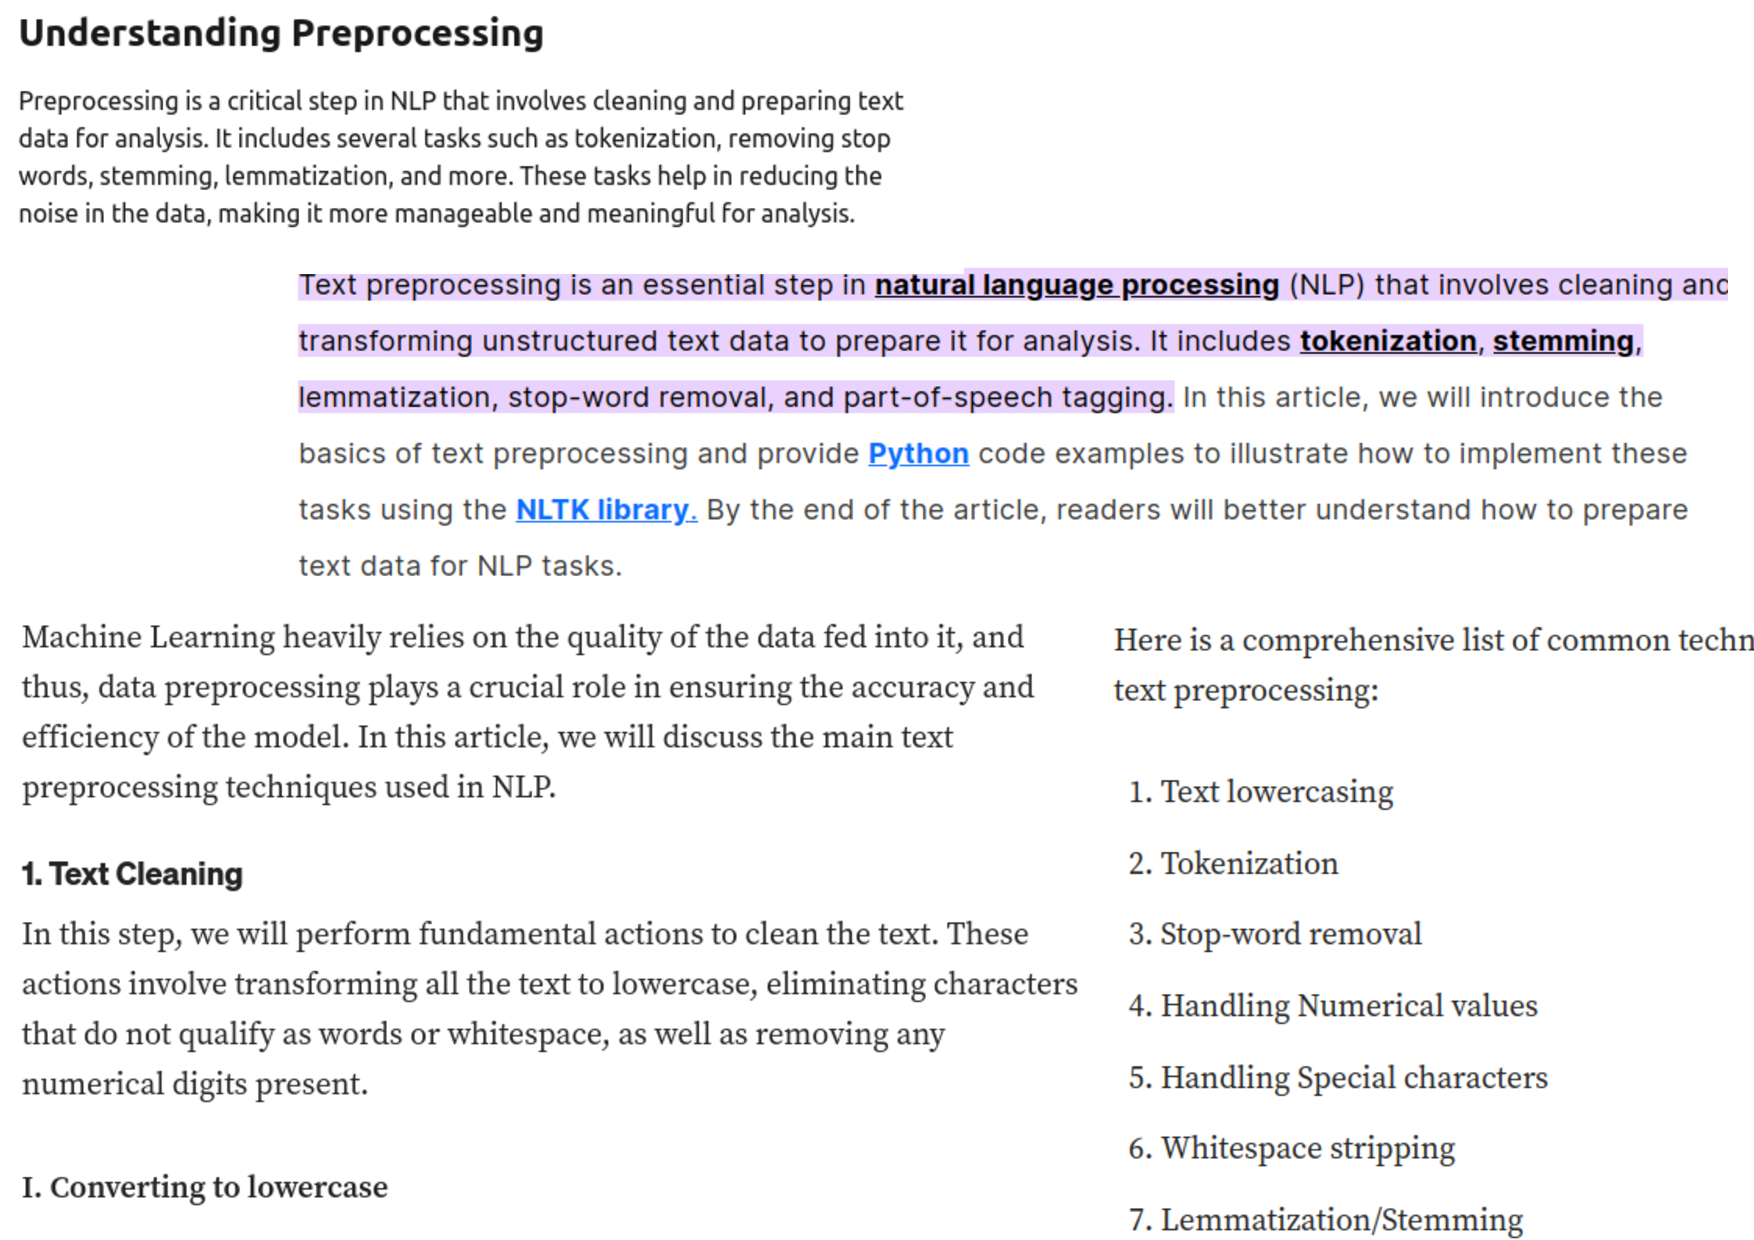
\includegraphics[width=1\textwidth]{./images/preprocess.pdf}
\end{figure}

\end{frame}

%%\begin{frame}{Outline}
%%\tableofcontents
%%\end{frame}

%% Sections create small transitions

\begin{frame}{Processing or Preprocessing}

\begin{block}{What is the difference?}
\begin{itemize}
\item Preprocessing steps seem harmless (but mandatory?)
\item Are "Processing" steps more noble?
\pause
\item Which ones are documented and justified?
\end{itemize}
\pause
Preprocessing steps are in fact full-fledged processing steps, since they have a non-negligible impact on subsequent operations \cite{Millour-2020}

\pause
From a design perspective:
\begin{itemize}
  \item They take time
  \item Do they focus attention on the right problems?
\pause
  \item Do they actually improve results?
\end{itemize}
\pause
\end{block}

\end{frame}

\begin{frame}{Which preprocessing steps are we talking about?}

\textit{In the literature there is no convention adopted, and each work tests some preprocessing techniques rather than others.}

\begin{itemize}
\item Lowercase letters.
\item Spelling Correction.
\pause
\item Removing HTML tags / URLs.
\pause
\item Removing punctuation.
\item Removing stop words.
\pause
\item Removing emojis.
\pause
\item Tokenization.
\item Stemming.
\item Lemmatization.
\end{itemize}
\pause
	\footnotesize{
How good is your tokenizer? on the monolingual performance of multilingual language models \cite{Rust-2020} 

Stemming impact on arabic text categorization performance: A survey (Al Anzi 2015)

	\textbf{Is text preprocessing still worth the time? A comparative survey on the influence of popular preprocessing methods} \dots \cite{Siino-2024}
	}
\end{frame}

\begin{frame}{A more detailed overview (Siino et al.)}
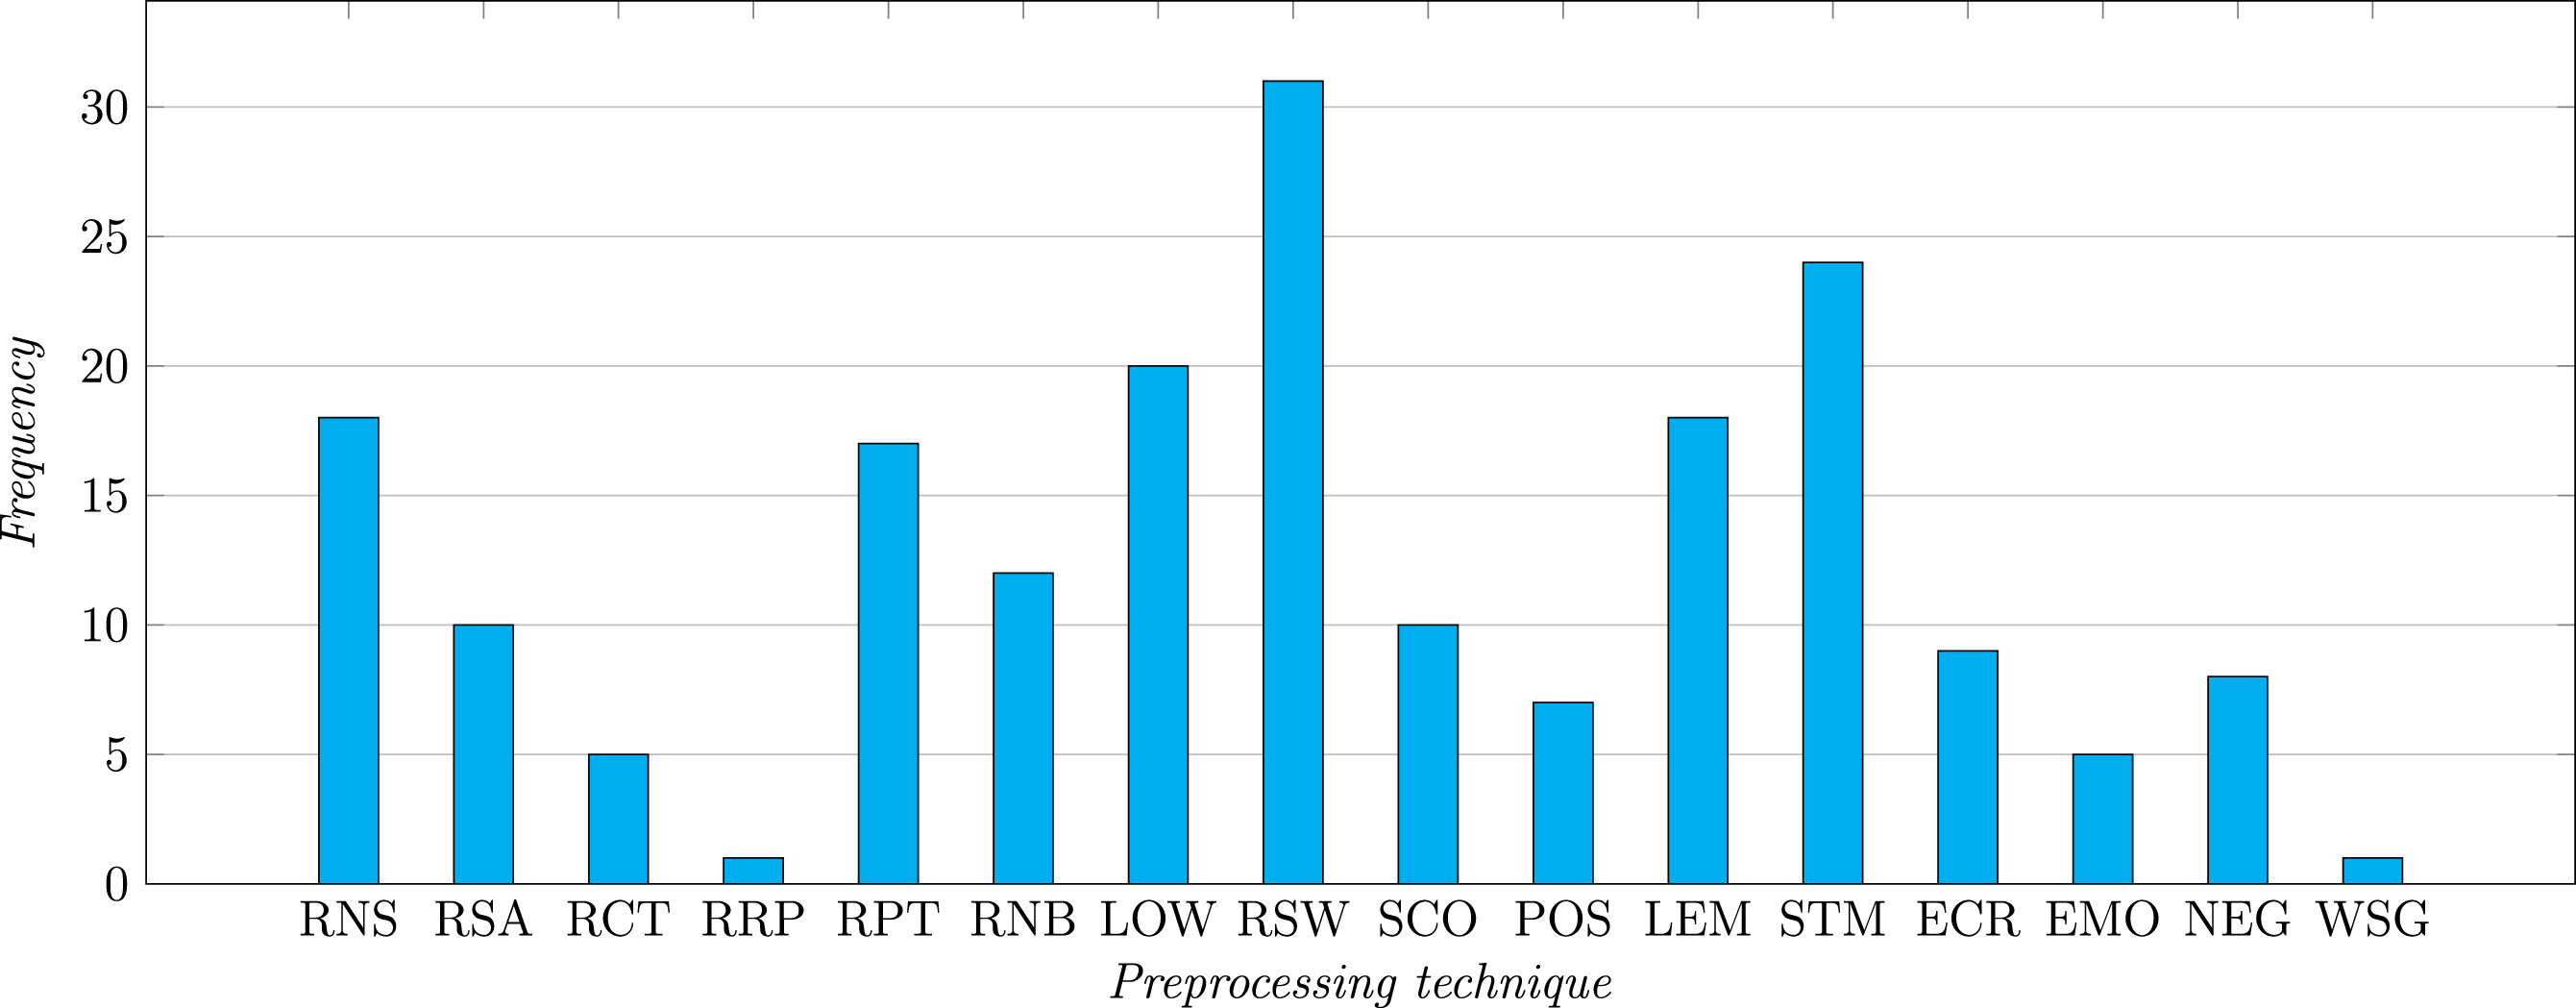
\includegraphics[width=.7\textwidth]{./images/preprocess_stats.png}
\begin{table}
\begin{tabular}{llll}
\textbf{ DON }&{ Do Nothing }&\textbf{  SCO }&{ Spelling Correction }\\
\textbf{ RNS }&{ Replace Noise }&\textbf{  POS }&{ Part-of-Speech Tagging }\\
\textbf{ RSA }&{ Replace Slang/Abbreviations }&\textbf{  LEM }&{ Lemmatization }\\
\textbf{ RCT }&{ Replace Contraction }&\textbf{  STM }&{ Stemming }\\
\textbf{ RRP }&{ Remove Repeated Punctuation }&\textbf{  ECR }&{ Remove Elongation }\\
\textbf{ RPT }&{ Removing Punctuation }&\textbf{  EMO }&{ Emoticon Handling }\\
\textbf{ RNB }&{ Remove Numbers }&\textbf{  NEG }&{ Negation Handling }\\
\textbf{ LOW }&{ Lowercasing }&\textbf{  WSG }&{ Word Segmentation  }\\
\textbf{ RSW }&{ Remove Stop Words }&\textbf{   }&{(some trending topic)  }\\
\end{tabular}
\end{table}

\end{frame}

\begin{frame}{Sentiment on Reviews \texttt{en} \cite{Siino-2024}}
\begin{figure}
\includegraphics[width=.6\textwidth]{./images/Res_siino.png}
\caption{Median accuracy over 5 runs + max difference. For each model, the best result is in bold, the worst in red.}
\end{figure}
\end{frame}

\begin{frame}{A more detailed overview (\texttt{en}) (Siino et al.)}
IMDB: Review Polarity, PCL: Press Condescending Language

FNS: Fake News, 20N: Forum Categorization
\includegraphics[width=.6\textwidth]{./images/Res_siino2.png}
\end{frame}

\begin{frame}{Figurative Language in Tweets \texttt{fr} \cite{Choi-2020}}
\begin{table}
\begin{scriptsize}
\begin{tabular}{|l|p{.5cm}|p{.5cm}|p{.5cm}|p{.5cm}|p{.5cm}|p{.5cm}|p{.5cm}|p{.5cm}|p{.5cm}|p{.5cm}|}
\hline
 & \multicolumn{2}{l|}{\textbf{\begin{tabular}[c]{@{}l@{}}Logistic \\ Regression\end{tabular}}} & \multicolumn{2}{l|}{\textbf{Decision Tree}} & \multicolumn{2}{l|}{\textbf{MNB}} & \multicolumn{2}{l|}{\textbf{KNN}} & \multicolumn{2}{l|}{\textbf{Random Forest}} \\ \hline
 & \textbf{Count} & \textbf{Tfidf} & \textbf{Count} & \textbf{Tfidf} & \textbf{Count} & \textbf{Tfidf} & \textbf{Count} & \textbf{Tfidf} & \textbf{Count} & \textbf{Tfidf} \\ \hline
\textbf{DON} & \textbf{50.20\ } & \textbf{52.03 } & \textbf{50.41 } & \textbf{42.89 } & \textbf{51.42 } & \textbf{52.24 } & \textbf{38.82 } & \textbf{45.73 } & \textbf{53.25 } & \textbf{51.22 } \\ \hline
\textbf{RPT} & 50.41  & 52.64  & 48.37 & 44.72  & 50.81  & 51.63  & 38.21  & 45.53 & \textbf{\color{blue}53.05}  & \textbf{\color{blue}52.64}  \\ \hline
\textbf{RSW} & \textbf{\color{blue}52.24 } & 53.86  & 45.93  & 44.11  & 51.22  & 52.24  & 37.40  & 44.31  & 50.00  & 50.20  \\ \hline
\textbf{ACC} & 49.59  & 52.64  & 49.39  & 43.29 & 51.02  & 52.03  & 35.16  & 45.53  & 52.44  & 52.03  \\ \hline
\textbf{\color{red}\textbf{URL}} & \textbf{\color{red}47.56 } & \textbf{\color{red}47.36 } & \textbf{\color{red}39.43 } & \textbf{\color{red}39.43 } & \textbf{\color{red}50.20 } & \textbf{\color{red}50.61 } & \textbf{\color{red}34.35 } & \textbf{\color{red}41.46 } & \textbf{\color{red}45.53 } & \textbf{\color{red}44.51 } \\ \hline
\textbf{\color{blue}\textbf{LEM}} & 50.20  & \textbf{\color{blue}54.07 } & \textbf{\color{blue}49.19}  & 44.72 & \textbf{\color{blue}52.24 } & \textbf{\color{blue}53.25 } & \textbf{\color{blue}39.02 } & 45.53  & 50.41  & 51.63  \\ \hline
\textbf{STM} & 51.63  & 53.86  & 48.37 & \textbf{\color{blue}45.93}  & 52.03  & 52.44 & 38.41  & \textbf{\color{blue}46.75 } & 52.44 & 51.42 \\ \hline
\end{tabular}
\caption{Average accuracy (in blue: best result, in red: worst result for each classifier)}
\end{scriptsize}
\end{table}
\end{frame}

\begin{frame}{Figurative Language in Tweets \texttt{fr} (Choi 2020)}
\begin{table}[!h]
\centering
\begin{small}
	\begin{tabular}{|p{1.8cm}|p{2.8cm}|p{1cm}|p{2.8cm}|p{1cm}|}
	\hline
    \textbf{Classifier}& \textbf{Count Vectorizer} & \textbf{Macro F1-score} & \textbf{Tfidf Vectorizer} & \textbf{Macro F1-score}\\
	\hline
	\textbf{Logistic Regression} & LEM, \mbox{RSW}	& 53.53  &	LEM, \mbox{RSW}, \mbox{RAC} & 54.35 \\
	\hline
	\textbf{Decision Tree}	& RPT, \mbox{accents}, \mbox{RAC}, \mbox{RSW}	& 49.59  & RAC, \mbox{RPT} & 48.58 \\
	\hline
	\textbf{MNB} & LEM, \mbox{RSW}, \mbox{RAC} & 54.59  & LEM, \mbox{RSW}, \mbox{RAC}	& {\color{blue}\textbf{55.89}}\\
	\hline
	\textbf{KNN} & RAC, \mbox{RSW}, \mbox{RPT}	& {\color{red}\textbf{38.20 }} & RAC, \mbox{RSW} & 47.35 \\
	\hline
	\textbf{Random Forest} & LEM, \mbox{RSW}, \mbox{accents}, \mbox{RAC} & 51.38  & LEM, \mbox{RSW}, \mbox{accents}, \mbox{RAC} & 53.25\\
	\hline
	\end{tabular}
\end{small}
\caption{Best macro F1-scores (in blue: best result, in red: worst result. Best result of DEFT2017: 65\%)}
\end{table}

\end{frame}

\begin{frame}{Combinations of preprocessing steps}
A comparative evaluation of pre-processing techniques and their interactions for twitter sentiment analysis \cite{Symeonidis-2018}
\pause

Influence of preprocessing on text classification – Application to tweet polarity classification \cite{Choi-2020}
\pause
\begin{block}{What do we learn?}
  \begin{itemize}
    \item Two preprocessing steps can interact negatively
    \item Performance gains tend to be asymptotic
\pause
    \item There is no universal “cocktail” that works regardless of:
     \begin{itemize}
        \item the task
        \item the type of texts
        \item the classifier
        \item the language model
    \end{itemize}
  \end{itemize}
\end{block}
\end{frame}

\begin{frame}{Let's put that in practice}

%TODO: add qrcode
%\fancyqr[classic]{https://github.com/rundimeco/Preprocessing_NLP}
	\small{
\url{https://github.com/rundimeco/Preprocessing_NLP} :

	\begin{itemize}
\item These slides (PDF)
\item A simple notebook illustrating multi-class classification:
\item \texttt{01\_run\_experiments\_simple\_task.ipynb} (Kaggle dataset)
\item Another example based on a well-known multilingual dataset (\texttt{corpus\_multi.zip}):
      \texttt{02\_DiagLang.ipynb}
\item We then experiment with a different dataset:
\item \small{\url{https://www.kaggle.com/datasets/suraj520/multi-task-learning}} (\texttt{03\_Sentiment\_analysis.ipynb})
\item The objective is to compare different classifiers and to understand:
        \begin{itemize}
\item which preprocessing steps are the most effective
\item how preprocessing effectiveness depends on the classifier
\item how it depends on the task, the type of text, and the language \dots
\end{itemize}
\end{itemize}
	}
\end{frame}


\begin{frame}[allowframebreaks]%{Références}
\setbeamerfont{bibliography entry title}{size=\scriptsize}
\bibliographystyle{apalike}
%\small{
\bibliography{biblio}
%}
\end{frame}

%% la biblio si besoin :
%%%\begin{frame}[allowframebreaks]{Références}
%%%
%%%%\bibliographystyle{unsrt}
%%%  \bibliographystyle{apalike}
%%%\scriptsize{
%%%\bibliography{biblio}}
%%%\end{frame}

\end{document}

\begin{frame}{}
\begin{block}{}
  \begin{itemize}
    \item
    \item
    \item
    \item
    \item
  \end{itemize}
\end{block}
\end{frame}




\end{document}
